\documentclass[twoside]{book}

% Packages required by doxygen
\usepackage{fixltx2e}
\usepackage{calc}
\usepackage{doxygen}
\usepackage[export]{adjustbox} % also loads graphicx
\usepackage{graphicx}
\usepackage[utf8]{inputenc}
\usepackage{makeidx}
\usepackage{multicol}
\usepackage{multirow}
\PassOptionsToPackage{warn}{textcomp}
\usepackage{textcomp}
\usepackage[nointegrals]{wasysym}
\usepackage[table]{xcolor}

% Font selection
\usepackage[T1]{fontenc}
\usepackage[scaled=.90]{helvet}
\usepackage{courier}
\usepackage{amssymb}
\usepackage{sectsty}
\renewcommand{\familydefault}{\sfdefault}
\allsectionsfont{%
  \fontseries{bc}\selectfont%
  \color{darkgray}%
}
\renewcommand{\DoxyLabelFont}{%
  \fontseries{bc}\selectfont%
  \color{darkgray}%
}
\newcommand{\+}{\discretionary{\mbox{\scriptsize$\hookleftarrow$}}{}{}}

% Page & text layout
\usepackage{geometry}
\geometry{%
  a4paper,%
  top=2.5cm,%
  bottom=2.5cm,%
  left=2.5cm,%
  right=2.5cm%
}
\tolerance=750
\hfuzz=15pt
\hbadness=750
\setlength{\emergencystretch}{15pt}
\setlength{\parindent}{0cm}
\setlength{\parskip}{0.2cm}
\makeatletter
\renewcommand{\paragraph}{%
  \@startsection{paragraph}{4}{0ex}{-1.0ex}{1.0ex}{%
    \normalfont\normalsize\bfseries\SS@parafont%
  }%
}
\renewcommand{\subparagraph}{%
  \@startsection{subparagraph}{5}{0ex}{-1.0ex}{1.0ex}{%
    \normalfont\normalsize\bfseries\SS@subparafont%
  }%
}
\makeatother

% Headers & footers
\usepackage{fancyhdr}
\pagestyle{fancyplain}
\fancyhead[LE]{\fancyplain{}{\bfseries\thepage}}
\fancyhead[CE]{\fancyplain{}{}}
\fancyhead[RE]{\fancyplain{}{\bfseries\leftmark}}
\fancyhead[LO]{\fancyplain{}{\bfseries\rightmark}}
\fancyhead[CO]{\fancyplain{}{}}
\fancyhead[RO]{\fancyplain{}{\bfseries\thepage}}
\fancyfoot[LE]{\fancyplain{}{}}
\fancyfoot[CE]{\fancyplain{}{}}
\fancyfoot[RE]{\fancyplain{}{\bfseries\scriptsize Generated on Fri Dec 11 2015 10\+:25\+:06 for C++\+Project by Doxygen }}
\fancyfoot[LO]{\fancyplain{}{\bfseries\scriptsize Generated on Fri Dec 11 2015 10\+:25\+:06 for C++\+Project by Doxygen }}
\fancyfoot[CO]{\fancyplain{}{}}
\fancyfoot[RO]{\fancyplain{}{}}
\renewcommand{\footrulewidth}{0.4pt}
\renewcommand{\chaptermark}[1]{%
  \markboth{#1}{}%
}
\renewcommand{\sectionmark}[1]{%
  \markright{\thesection\ #1}%
}

% Indices & bibliography
\usepackage{natbib}
\usepackage[titles]{tocloft}
\setcounter{tocdepth}{3}
\setcounter{secnumdepth}{5}
\makeindex

% Hyperlinks (required, but should be loaded last)
\usepackage{ifpdf}
\ifpdf
  \usepackage[pdftex,pagebackref=true]{hyperref}
\else
  \usepackage[ps2pdf,pagebackref=true]{hyperref}
\fi
\hypersetup{%
  colorlinks=true,%
  linkcolor=blue,%
  citecolor=blue,%
  unicode%
}

% Custom commands
\newcommand{\clearemptydoublepage}{%
  \newpage{\pagestyle{empty}\cleardoublepage}%
}


%===== C O N T E N T S =====

\begin{document}

% Titlepage & ToC
\hypersetup{pageanchor=false,
             bookmarks=true,
             bookmarksnumbered=true,
             pdfencoding=unicode
            }
\pagenumbering{roman}
\begin{titlepage}
\vspace*{7cm}
\begin{center}%
{\Large C++\+Project }\\
\vspace*{1cm}
{\large Generated by Doxygen 1.8.10}\\
\vspace*{0.5cm}
{\small Fri Dec 11 2015 10:25:06}\\
\end{center}
\end{titlepage}
\clearemptydoublepage
\tableofcontents
\clearemptydoublepage
\pagenumbering{arabic}
\hypersetup{pageanchor=true}

%--- Begin generated contents ---
\chapter{Main Page}
\label{index}\hypertarget{index}{}Library for solving differential equations of the type dy/dt=f(y,t). It can handle non-\/linear differential equation of first order. ~\newline
 It has three different ways of inputting the righandside function f(y,t), which are all implemented as subclasses of the abstract class \char`\"{}righthandside\char`\"{}\+:

1)As a pointer to a Generic User defined function, though the use of the \char`\"{}\+Generic\+Function\char`\"{} class. The user can specify f(y,t) and its gradient. ~\newline
 2)As a generic polynomial function of maximum grade 4, with the use of \char`\"{}\+Polynomial\char`\"{} class. The function must be of the form\+: a+b$\ast$y+c$\ast$y$^\wedge$2+d$\ast$y$^\wedge$3+e$\ast$y$^\wedge$4 ~\newline
 3)As a function including a sine and a cosine of the form\+: a$\ast$sin(c$\ast$y)+b$\ast$cos(d$\ast$y). This is done with the \char`\"{}\+Sin\+Cos\char`\"{} class. ~\newline


Six different solvers can be used, all programmed as derived classes from the \char`\"{}\+Abstract\+Ode\+Solver\char`\"{} class\+:

1)\char`\"{}\+Forward\+Euler\+Solver\char`\"{}\+: Solves the differential equation using forward Euler method ~\newline
 2)\char`\"{}\+Backward\+Euler\+Solver\char`\"{}\+: Solves the differential equation using backward Euler method ~\newline
 3)\char`\"{}\+Twostep\+Solver\char`\"{}\+: Solves the differential equation using two step Adam Bashforth method ~\newline
 4)\char`\"{}\+Threestep\+Solver\char`\"{}\+: Solves the differential equation using three step Adam Bashforth method ~\newline
 5)\char`\"{}\+Fourstep\+Solver\char`\"{}\+: Solves the differential equation using four step Adam Bashforth method ~\newline
 6)\char`\"{}\+Runge\+Kutta4\+Solver\char`\"{}\+: Solves the differential equation using fourth order Runge-\/\+Kutta method ~\newline


The library was developed by Francesco Mancino as a project for the course \char`\"{}\+Programming concepts in scientific computing\char`\"{} at E\+P\+F\+L.

Contact\+: \href{mailto:francesco.mancino@EPFL.ch}{\tt francesco.\+mancino@\+E\+P\+F\+L.\+ch} 
\chapter{Hierarchical Index}
\section{Class Hierarchy}
This inheritance list is sorted roughly, but not completely, alphabetically\+:\begin{DoxyCompactList}
\item \contentsline{section}{Abstract\+Ode\+Solver}{\pageref{class_abstract_ode_solver}}{}
\begin{DoxyCompactList}
\item \contentsline{section}{Backward\+Euler\+Solver}{\pageref{class_backward_euler_solver}}{}
\item \contentsline{section}{Forward\+Euler\+Solver}{\pageref{class_forward_euler_solver}}{}
\item \contentsline{section}{Four\+Step\+Solver}{\pageref{class_four_step_solver}}{}
\item \contentsline{section}{Runge\+Kutta4\+Solver}{\pageref{class_runge_kutta4_solver}}{}
\item \contentsline{section}{Three\+Step\+Solver}{\pageref{class_three_step_solver}}{}
\item \contentsline{section}{Two\+Step\+Solver}{\pageref{class_two_step_solver}}{}
\end{DoxyCompactList}
\item \contentsline{section}{Righthandside}{\pageref{class_righthandside}}{}
\begin{DoxyCompactList}
\item \contentsline{section}{Generic\+Function}{\pageref{class_generic_function}}{}
\item \contentsline{section}{Polynomial$<$ T $>$}{\pageref{class_polynomial}}{}
\item \contentsline{section}{Sin\+Cos$<$ T $>$}{\pageref{class_sin_cos}}{}
\end{DoxyCompactList}
\end{DoxyCompactList}

\chapter{Class Index}
\section{Class List}
Here are the classes, structs, unions and interfaces with brief descriptions\+:\begin{DoxyCompactList}
\item\contentsline{section}{\hyperlink{class_abstract_ode_solver}{Abstract\+Ode\+Solver} \\*Abstract Base class for the family of methods for solving O\+D\+E of the form dy/dt=f(y,t) }{\pageref{class_abstract_ode_solver}}{}
\item\contentsline{section}{\hyperlink{class_backward_euler_solver}{Backward\+Euler\+Solver} \\*Class that implements Backward Eulers method to solve a O\+D\+E of the form\+: dy/dt=f(y,t) }{\pageref{class_backward_euler_solver}}{}
\item\contentsline{section}{\hyperlink{class_forward_euler_solver}{Forward\+Euler\+Solver} \\*Class that implements Forward Eulers method to solve a O\+D\+E of the form\+: dy/dt=f(y,t) }{\pageref{class_forward_euler_solver}}{}
\item\contentsline{section}{\hyperlink{class_four_step_solver}{Four\+Step\+Solver} \\*Class that implements Four Step Adam Bashworts Method to solve a O\+D\+E of the form\+: dy/dt=f(y,t) }{\pageref{class_four_step_solver}}{}
\item\contentsline{section}{\hyperlink{class_generic_function}{Generic\+Function} \\*Class that allows the user to specify a generic function and its gradient, with the use of function pointers, as the right hand side of the O\+D\+E }{\pageref{class_generic_function}}{}
\item\contentsline{section}{\hyperlink{class_polynomial}{Polynomial$<$ T $>$} \\*Class that allows the user to specify a polynomial of grade 2 up to 4, in the form\+: a+b$\ast$x+c$\ast$x$^\wedge$2+d$\ast$x$^\wedge$3+e$\ast$x$^\wedge$4, as the right hand side of the O\+D\+E }{\pageref{class_polynomial}}{}
\item\contentsline{section}{\hyperlink{class_righthandside}{Righthandside} \\*Abstract Base class of the family of possible right hand side functions f(y,t) in the O\+D\+E dy/dt=f(y,t) }{\pageref{class_righthandside}}{}
\item\contentsline{section}{\hyperlink{class_runge_kutta4_solver}{Runge\+Kutta4\+Solver} \\*Class that implements 4th order Runge-\/\+Kutta method to solve a O\+D\+E of the form\+: dy/dt=f(y,t) }{\pageref{class_runge_kutta4_solver}}{}
\item\contentsline{section}{\hyperlink{class_sin_cos}{Sin\+Cos$<$ T $>$} \\*Class that allows the user to specify a function of the type f(y,t)=a$\ast$sin(c$\ast$y)+b$\ast$cos(d$\ast$y) for the right hand side of the O\+D\+E }{\pageref{class_sin_cos}}{}
\item\contentsline{section}{\hyperlink{class_three_step_solver}{Three\+Step\+Solver} \\*Class that implements Four Three Adam Bashworts Method to solve a O\+D\+E of the form\+: dy/dt=f(y,t) }{\pageref{class_three_step_solver}}{}
\item\contentsline{section}{\hyperlink{class_two_step_solver}{Two\+Step\+Solver} \\*Class that implements Two Step Adam Bashworts Method to solve a O\+D\+E of the form\+: dy/dt=f(y,t) }{\pageref{class_two_step_solver}}{}
\end{DoxyCompactList}

\chapter{Class Documentation}
\hypertarget{class_abstract_ode_solver}{}\section{Abstract\+Ode\+Solver Class Reference}
\label{class_abstract_ode_solver}\index{Abstract\+Ode\+Solver@{Abstract\+Ode\+Solver}}


Abstract Base class for the family of methods for solving O\+D\+E of the form dy/dt=f(y,t).  




{\ttfamily \#include $<$Abstract\+Ode\+Solver.\+hpp$>$}

Inheritance diagram for Abstract\+Ode\+Solver\+:\begin{figure}[H]
\begin{center}
\leavevmode
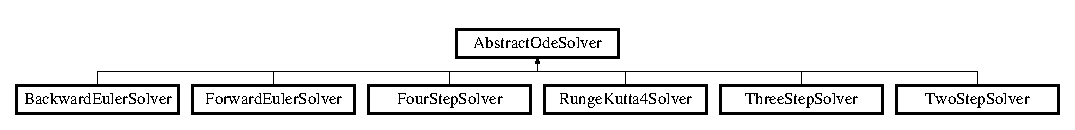
\includegraphics[height=1.305361cm]{class_abstract_ode_solver}
\end{center}
\end{figure}
\subsection*{Public Member Functions}
\begin{DoxyCompactItemize}
\item 
\hypertarget{class_abstract_ode_solver_a67a8c0665a9b5d2de74a1307087f23c4}{}void \hyperlink{class_abstract_ode_solver_a67a8c0665a9b5d2de74a1307087f23c4}{Set\+Number\+Steps} (int n)\label{class_abstract_ode_solver_a67a8c0665a9b5d2de74a1307087f23c4}

\begin{DoxyCompactList}\small\item\em Sets the number of steps taken by the O\+D\+E solver . \end{DoxyCompactList}\item 
\hypertarget{class_abstract_ode_solver_aa538dd3bcac6ba5c784dec442333686f}{}void \hyperlink{class_abstract_ode_solver_aa538dd3bcac6ba5c784dec442333686f}{Set\+Time\+Interval} (double t0, double t1)\label{class_abstract_ode_solver_aa538dd3bcac6ba5c784dec442333686f}

\begin{DoxyCompactList}\small\item\em Sets the time interval of the solution. \end{DoxyCompactList}\item 
\hypertarget{class_abstract_ode_solver_a0340b4da640c8c9131363d0525d9223b}{}void \hyperlink{class_abstract_ode_solver_a0340b4da640c8c9131363d0525d9223b}{Set\+Initial\+Value} (double y0)\label{class_abstract_ode_solver_a0340b4da640c8c9131363d0525d9223b}

\begin{DoxyCompactList}\small\item\em Sets the initial value of the solution. \end{DoxyCompactList}\item 
\hypertarget{class_abstract_ode_solver_a6a7f536dd540c74189b2780ef88f4150}{}int {\bfseries Get\+Number\+Steps} ()\label{class_abstract_ode_solver_a6a7f536dd540c74189b2780ef88f4150}

\item 
\hypertarget{class_abstract_ode_solver_a6896791ac972393fb2fe55a974a9e4df}{}double {\bfseries Get\+Initial\+Time} ()\label{class_abstract_ode_solver_a6896791ac972393fb2fe55a974a9e4df}

\item 
\hypertarget{class_abstract_ode_solver_ae1d50acb9cc96e75e05bc1361a0443a6}{}double {\bfseries Get\+Final\+Time} ()\label{class_abstract_ode_solver_ae1d50acb9cc96e75e05bc1361a0443a6}

\item 
\hypertarget{class_abstract_ode_solver_a849db045f2d9f873c89f3ffd568c4f2f}{}double {\bfseries Get\+Initial\+Value} ()\label{class_abstract_ode_solver_a849db045f2d9f873c89f3ffd568c4f2f}

\item 
virtual void \hyperlink{class_abstract_ode_solver_ad7d73b20e9ce5c8f3aab1a15bebe3e4c}{Solve\+Equation} (\hyperlink{class_righthandside}{Righthandside} $\ast$f, std\+::ostream \&stream)=0
\end{DoxyCompactItemize}


\subsection{Detailed Description}
Abstract Base class for the family of methods for solving O\+D\+E of the form dy/dt=f(y,t). 

Abstrac\+Ode\+Solver.\+cpp

Created on\+: Dic, 2015 \begin{DoxyVerb}Author: Francesco Mancino
\end{DoxyVerb}


Description\+: Abstract Base class for the family of methods for solving O\+D\+E of the form dy/dt=f(y,t). The possible methods are defined as derived classes from this class. 

\subsection{Member Function Documentation}
\hypertarget{class_abstract_ode_solver_ad7d73b20e9ce5c8f3aab1a15bebe3e4c}{}\index{Abstract\+Ode\+Solver@{Abstract\+Ode\+Solver}!Solve\+Equation@{Solve\+Equation}}
\index{Solve\+Equation@{Solve\+Equation}!Abstract\+Ode\+Solver@{Abstract\+Ode\+Solver}}
\subsubsection[{Solve\+Equation(\+Righthandside $\ast$f, std\+::ostream \&stream)=0}]{\setlength{\rightskip}{0pt plus 5cm}virtual void Abstract\+Ode\+Solver\+::\+Solve\+Equation (
\begin{DoxyParamCaption}
\item[{{\bf Righthandside} $\ast$}]{f, }
\item[{std\+::ostream \&}]{stream}
\end{DoxyParamCaption}
)\hspace{0.3cm}{\ttfamily [pure virtual]}}\label{class_abstract_ode_solver_ad7d73b20e9ce5c8f3aab1a15bebe3e4c}
Virtual function the solves the O\+D\+E with initial conditions, Time interval, and number of steps specified in the methods of \char`\"{}\+Abstact\+Ode\+Solver\char`\"{}. The first input is the right hand side of the O\+D\+E, also a class, and the second input is the file in which the solution will be saved. 

Implemented in \hyperlink{class_backward_euler_solver_ad800861c582a920b98288d65e0f68d45}{Backward\+Euler\+Solver}, \hyperlink{class_forward_euler_solver_af1d0ccddde281d136a99362743c80fe7}{Forward\+Euler\+Solver}, \hyperlink{class_four_step_solver_a78b7b6af19731e904c4cdd31b5641aa2}{Four\+Step\+Solver}, \hyperlink{class_runge_kutta4_solver_acd37986ea1784f8ee4ae27f1614b06b8}{Runge\+Kutta4\+Solver}, \hyperlink{class_two_step_solver_ae52e8c2313e8f9fa617d13b7ed83284e}{Two\+Step\+Solver}, and \hyperlink{class_three_step_solver_a5c84debbe6e3497ab3c4b796e1f92cee}{Three\+Step\+Solver}.



The documentation for this class was generated from the following files\+:\begin{DoxyCompactItemize}
\item 
/\+Users/macair/\+Documents/projectode/Abstract\+Ode\+Solver.\+hpp\item 
/\+Users/macair/\+Documents/projectode/Abstract\+Ode\+Solver.\+cpp\end{DoxyCompactItemize}

\hypertarget{class_backward_euler_solver}{}\section{Backward\+Euler\+Solver Class Reference}
\label{class_backward_euler_solver}\index{Backward\+Euler\+Solver@{Backward\+Euler\+Solver}}


{\ttfamily \#include $<$Backward\+Euler\+Solver.\+hpp$>$}

Inheritance diagram for Backward\+Euler\+Solver\+:\begin{figure}[H]
\begin{center}
\leavevmode
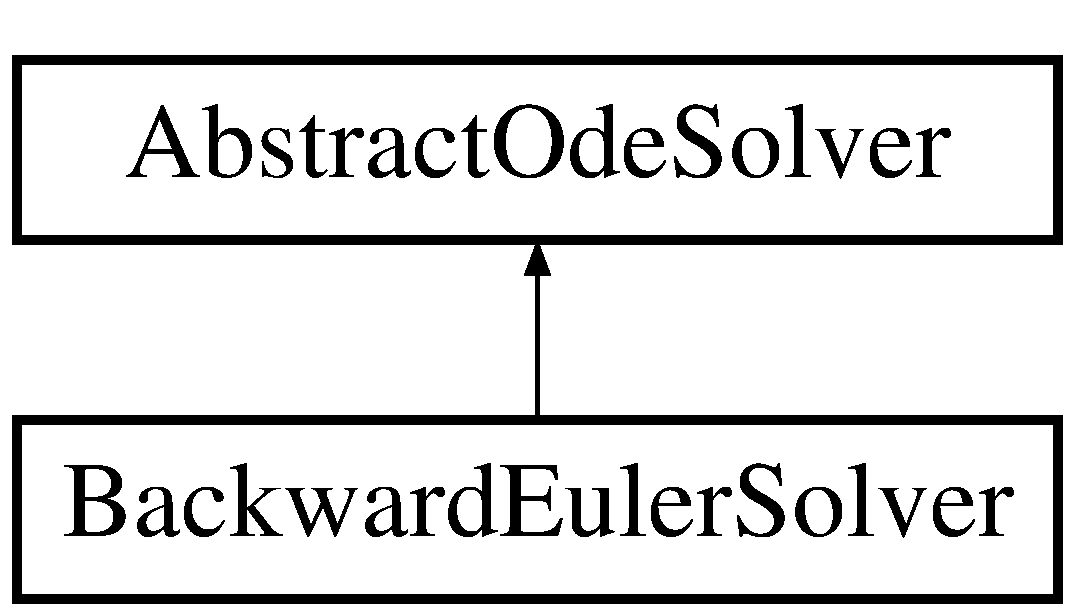
\includegraphics[height=2.000000cm]{class_backward_euler_solver}
\end{center}
\end{figure}
\subsection*{Public Member Functions}
\begin{DoxyCompactItemize}
\item 
virtual void \hyperlink{class_backward_euler_solver_ad800861c582a920b98288d65e0f68d45}{Solve\+Equation} (\hyperlink{class_righthandside}{Righthandside} $\ast$f, std\+::ostream \&stream)
\end{DoxyCompactItemize}


\subsection{Detailed Description}
Backward\+Eulersolver.\+cpp

Created on\+: Dic, 2015 \begin{DoxyVerb}Author: Francesco Mancino
\end{DoxyVerb}


Description\+: Class that implements Backward Eulers method to solve a O\+D\+E of the form\+: dy/dt=f(y,t). It is derived from the abstract class \hyperlink{class_abstract_ode_solver}{Abstract\+Ode\+Solver}. To Solve the equation arising due to the fact that Backward Eulers method is implicit, Newtons method is used if the gradient is specified and the secant method is used it the gradient is not specified. 

\subsection{Member Function Documentation}
\hypertarget{class_backward_euler_solver_ad800861c582a920b98288d65e0f68d45}{}\index{Backward\+Euler\+Solver@{Backward\+Euler\+Solver}!Solve\+Equation@{Solve\+Equation}}
\index{Solve\+Equation@{Solve\+Equation}!Backward\+Euler\+Solver@{Backward\+Euler\+Solver}}
\subsubsection[{Solve\+Equation(\+Righthandside $\ast$f, std\+::ostream \&stream)}]{\setlength{\rightskip}{0pt plus 5cm}void Backward\+Euler\+Solver\+::\+Solve\+Equation (
\begin{DoxyParamCaption}
\item[{{\bf Righthandside} $\ast$}]{f, }
\item[{std\+::ostream \&}]{stream}
\end{DoxyParamCaption}
)\hspace{0.3cm}{\ttfamily [virtual]}}\label{class_backward_euler_solver_ad800861c582a920b98288d65e0f68d45}
Virtual function the solves the O\+D\+E with initial conditions, Time interval, and number of steps specified in the methods of \char`\"{}\+Abstact\+Ode\+Solver\char`\"{}. The first input is the right hand side of the O\+D\+E, also a class, and the second input is the file in which the solution will be saved. 

Implements \hyperlink{class_abstract_ode_solver_ad7d73b20e9ce5c8f3aab1a15bebe3e4c}{Abstract\+Ode\+Solver}.



The documentation for this class was generated from the following files\+:\begin{DoxyCompactItemize}
\item 
/\+Users/macair/\+Documents/projectode/Backward\+Euler\+Solver.\+hpp\item 
/\+Users/macair/\+Documents/projectode/Backward\+Euler\+Solver.\+cpp\end{DoxyCompactItemize}

\hypertarget{class_forward_euler_solver}{}\section{Forward\+Euler\+Solver Class Reference}
\label{class_forward_euler_solver}\index{Forward\+Euler\+Solver@{Forward\+Euler\+Solver}}


{\ttfamily \#include $<$Forward\+Euler\+Solver.\+hpp$>$}

Inheritance diagram for Forward\+Euler\+Solver\+:\begin{figure}[H]
\begin{center}
\leavevmode
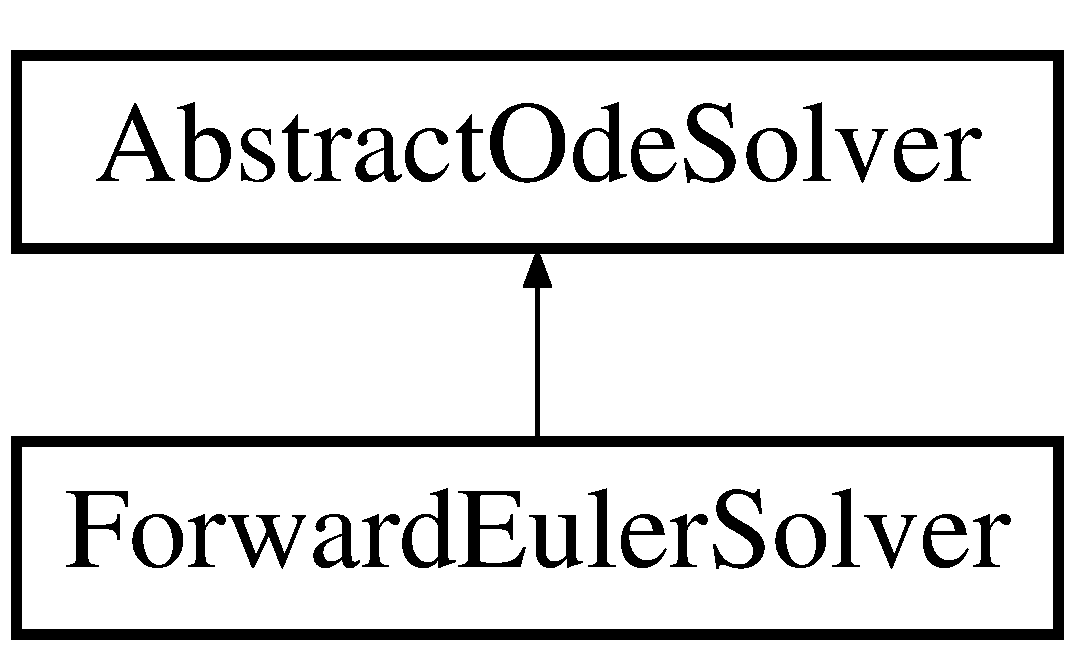
\includegraphics[height=2.000000cm]{class_forward_euler_solver}
\end{center}
\end{figure}
\subsection*{Public Member Functions}
\begin{DoxyCompactItemize}
\item 
\hyperlink{class_forward_euler_solver_a56271b4e9c08874b64e20981f4004294}{Forward\+Euler\+Solver} ()
\item 
virtual void \hyperlink{class_forward_euler_solver_af1d0ccddde281d136a99362743c80fe7}{Solve\+Equation} (\hyperlink{class_righthandside}{Righthandside} $\ast$f, std\+::ostream \&stream)
\end{DoxyCompactItemize}


\subsection{Detailed Description}
\hyperlink{_forward_euler_solver_8hpp_source}{Forward\+Eulersolver.\+hpp}

Created on\+: Dic, 2015 \begin{DoxyVerb}Author: Francesco Mancino
\end{DoxyVerb}


Description\+: Class that implements Forward Eulers method to solve a O\+D\+E of the form\+: dy/dt=f(y,t). It is derived from the abstract class \hyperlink{class_abstract_ode_solver}{Abstract\+Ode\+Solver}. 

\subsection{Constructor \& Destructor Documentation}
\hypertarget{class_forward_euler_solver_a56271b4e9c08874b64e20981f4004294}{}\index{Forward\+Euler\+Solver@{Forward\+Euler\+Solver}!Forward\+Euler\+Solver@{Forward\+Euler\+Solver}}
\index{Forward\+Euler\+Solver@{Forward\+Euler\+Solver}!Forward\+Euler\+Solver@{Forward\+Euler\+Solver}}
\subsubsection[{Forward\+Euler\+Solver()}]{\setlength{\rightskip}{0pt plus 5cm}Forward\+Euler\+Solver\+::\+Forward\+Euler\+Solver (
\begin{DoxyParamCaption}
{}
\end{DoxyParamCaption}
)}\label{class_forward_euler_solver_a56271b4e9c08874b64e20981f4004294}
\hyperlink{_forward_euler_solver_8hpp_source}{Forward\+Eulersolver.\+hpp} Created on\+: Dic, 2015 Author\+: Francesco Mancino Description\+: Class that implements Forward Eulers method to solve a O\+D\+E of the form\+: dy/dt=f(y,t). It is derived from the abstract class \hyperlink{class_abstract_ode_solver}{Abstract\+Ode\+Solver}. 

\subsection{Member Function Documentation}
\hypertarget{class_forward_euler_solver_af1d0ccddde281d136a99362743c80fe7}{}\index{Forward\+Euler\+Solver@{Forward\+Euler\+Solver}!Solve\+Equation@{Solve\+Equation}}
\index{Solve\+Equation@{Solve\+Equation}!Forward\+Euler\+Solver@{Forward\+Euler\+Solver}}
\subsubsection[{Solve\+Equation(\+Righthandside $\ast$f, std\+::ostream \&stream)}]{\setlength{\rightskip}{0pt plus 5cm}void Forward\+Euler\+Solver\+::\+Solve\+Equation (
\begin{DoxyParamCaption}
\item[{{\bf Righthandside} $\ast$}]{f, }
\item[{std\+::ostream \&}]{stream}
\end{DoxyParamCaption}
)\hspace{0.3cm}{\ttfamily [virtual]}}\label{class_forward_euler_solver_af1d0ccddde281d136a99362743c80fe7}
Virtual function the solves the O\+D\+E with initial conditions, Time interval, and number of steps specified in the methods of \char`\"{}\+Abstact\+Ode\+Solver\char`\"{}. The first input is the right hand side of the O\+D\+E, also a class, and the second input is the file in which the solution will be saved. 

Implements \hyperlink{class_abstract_ode_solver_ad7d73b20e9ce5c8f3aab1a15bebe3e4c}{Abstract\+Ode\+Solver}.



The documentation for this class was generated from the following files\+:\begin{DoxyCompactItemize}
\item 
/\+Users/macair/\+Documents/projectode/Forward\+Euler\+Solver.\+hpp\item 
/\+Users/macair/\+Documents/projectode/Forward\+Euler\+Solver.\+cpp\end{DoxyCompactItemize}

\hypertarget{class_four_step_solver}{}\section{Four\+Step\+Solver Class Reference}
\label{class_four_step_solver}\index{Four\+Step\+Solver@{Four\+Step\+Solver}}


Class that implements Four Step Adam Bashworts Method to solve a O\+D\+E of the form\+: dy/dt=f(y,t).  




{\ttfamily \#include $<$Four\+Step\+Solver.\+hpp$>$}

Inheritance diagram for Four\+Step\+Solver\+:\begin{figure}[H]
\begin{center}
\leavevmode
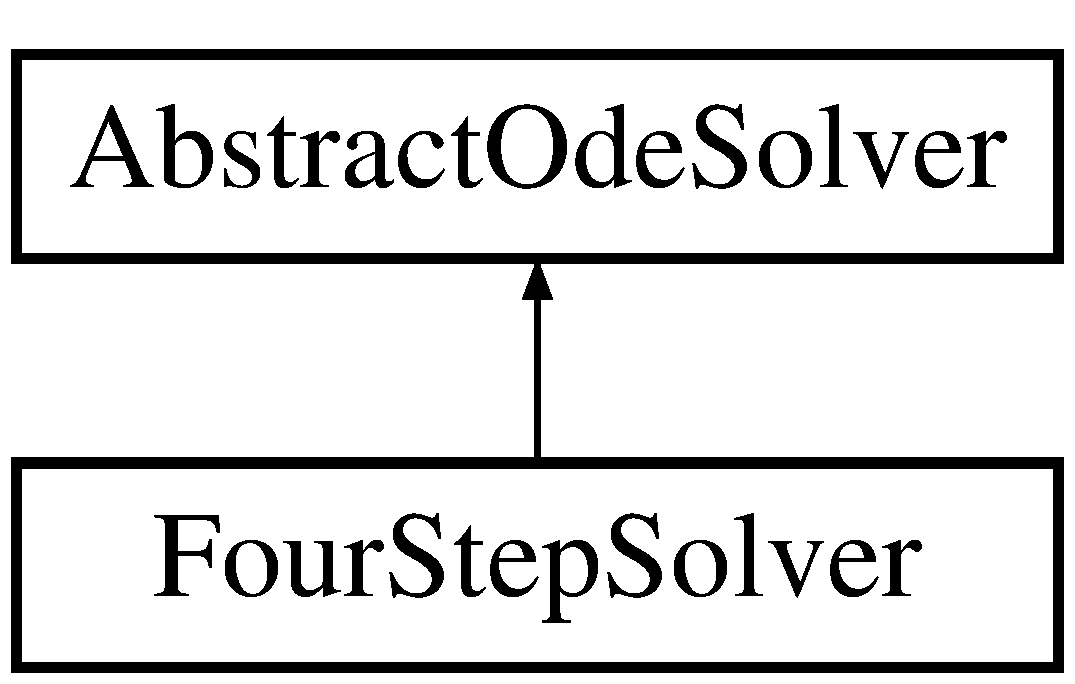
\includegraphics[height=2.000000cm]{class_four_step_solver}
\end{center}
\end{figure}
\subsection*{Public Member Functions}
\begin{DoxyCompactItemize}
\item 
virtual void \hyperlink{class_four_step_solver_a78b7b6af19731e904c4cdd31b5641aa2}{Solve\+Equation} (\hyperlink{class_righthandside}{Righthandside} $\ast$f, std\+::ostream \&stream)
\end{DoxyCompactItemize}


\subsection{Detailed Description}
Class that implements Four Step Adam Bashworts Method to solve a O\+D\+E of the form\+: dy/dt=f(y,t). 

Four\+Step\+Solver.\+cpp

Created on\+: Dic, 2015 \begin{DoxyVerb}Author: Francesco Mancino
\end{DoxyVerb}


Description\+: Class that implements Four Step Adam Bashworts Method to solve a O\+D\+E of the form\+: dy/dt=f(y,t). It is derived from the abstract class \hyperlink{class_abstract_ode_solver}{Abstract\+Ode\+Solver}. 

\subsection{Member Function Documentation}
\hypertarget{class_four_step_solver_a78b7b6af19731e904c4cdd31b5641aa2}{}\index{Four\+Step\+Solver@{Four\+Step\+Solver}!Solve\+Equation@{Solve\+Equation}}
\index{Solve\+Equation@{Solve\+Equation}!Four\+Step\+Solver@{Four\+Step\+Solver}}
\subsubsection[{Solve\+Equation(\+Righthandside $\ast$f, std\+::ostream \&stream)}]{\setlength{\rightskip}{0pt plus 5cm}void Four\+Step\+Solver\+::\+Solve\+Equation (
\begin{DoxyParamCaption}
\item[{{\bf Righthandside} $\ast$}]{f, }
\item[{std\+::ostream \&}]{stream}
\end{DoxyParamCaption}
)\hspace{0.3cm}{\ttfamily [virtual]}}\label{class_four_step_solver_a78b7b6af19731e904c4cdd31b5641aa2}
Virtual function the solves the O\+D\+E with initial conditions, Time interval, and number of steps specified in the methods of \char`\"{}\+Abstact\+Ode\+Solver\char`\"{}. The first input is the right hand side of the O\+D\+E, also a class, and the second input is the file in which the solution will be saved. 

Implements \hyperlink{class_abstract_ode_solver_ad7d73b20e9ce5c8f3aab1a15bebe3e4c}{Abstract\+Ode\+Solver}.



The documentation for this class was generated from the following files\+:\begin{DoxyCompactItemize}
\item 
/\+Users/macair/\+Documents/projectode/Four\+Step\+Solver.\+hpp\item 
/\+Users/macair/\+Documents/projectode/Four\+Step\+Solver.\+cpp\end{DoxyCompactItemize}

\hypertarget{class_generic_function}{}\section{Generic\+Function Class Reference}
\label{class_generic_function}\index{Generic\+Function@{Generic\+Function}}


Class that allows the user to specify a generic function and its gradient, with the use of function pointers, as the right hand side of the O\+D\+E.  




{\ttfamily \#include $<$Generic\+Function.\+hpp$>$}

Inheritance diagram for Generic\+Function\+:\begin{figure}[H]
\begin{center}
\leavevmode
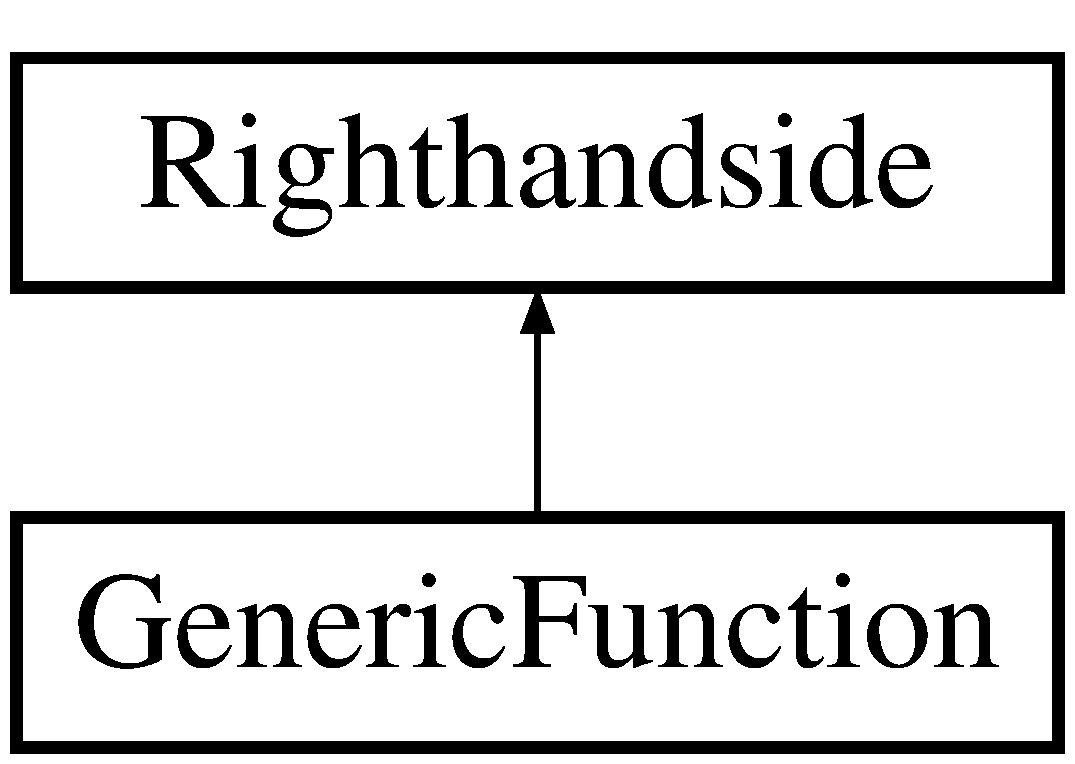
\includegraphics[height=2.000000cm]{class_generic_function}
\end{center}
\end{figure}
\subsection*{Public Member Functions}
\begin{DoxyCompactItemize}
\item 
\hypertarget{class_generic_function_a74e9aaff47e0bba83c0d0ad3f60b1ec5}{}\hyperlink{class_generic_function_a74e9aaff47e0bba83c0d0ad3f60b1ec5}{Generic\+Function} (double($\ast$f)(double y, double t))\label{class_generic_function_a74e9aaff47e0bba83c0d0ad3f60b1ec5}

\begin{DoxyCompactList}\small\item\em Constructor if you have only the function. \end{DoxyCompactList}\item 
\hypertarget{class_generic_function_a251276ed4f9512a284257e3965a18207}{}\hyperlink{class_generic_function_a251276ed4f9512a284257e3965a18207}{Generic\+Function} (double($\ast$f)(double y, double t), double($\ast$g)(double y, double t))\label{class_generic_function_a251276ed4f9512a284257e3965a18207}

\begin{DoxyCompactList}\small\item\em Constructor if you have function and gradient. \end{DoxyCompactList}\item 
\hypertarget{class_generic_function_ab6ff4fd2c397f0d57c96903277037c7e}{}virtual double \hyperlink{class_generic_function_ab6ff4fd2c397f0d57c96903277037c7e}{value} (double y, double t) const \label{class_generic_function_ab6ff4fd2c397f0d57c96903277037c7e}

\begin{DoxyCompactList}\small\item\em Virtual function to get the value of the function on the right hand side, f(y,t) for a specific y and t. \end{DoxyCompactList}\item 
\hypertarget{class_generic_function_afe74d7deb46708999a9d01514589f16b}{}virtual double \hyperlink{class_generic_function_afe74d7deb46708999a9d01514589f16b}{gradient} (double y, double t) const \label{class_generic_function_afe74d7deb46708999a9d01514589f16b}

\begin{DoxyCompactList}\small\item\em Virtual function to get the value gradient of the function on the right hand side, f\textquotesingle{}(y,t) for a specific y and t. \end{DoxyCompactList}\end{DoxyCompactItemize}


\subsection{Detailed Description}
Class that allows the user to specify a generic function and its gradient, with the use of function pointers, as the right hand side of the O\+D\+E. 

\hyperlink{_generic_function_8hpp_source}{Generic\+Function.\+hpp}

Created on\+: Dic, 2015 \begin{DoxyVerb}Author: Francesco Mancino
\end{DoxyVerb}


Description\+: Derived class from \hyperlink{class_righthandside}{Righthandside}. Allows the user to specify a generic function and its gradient, with the use of function pointers. The choice is given as to whether to specify the gradient or not, thought the use of two different constructors. 

The documentation for this class was generated from the following files\+:\begin{DoxyCompactItemize}
\item 
/\+Users/macair/\+Documents/projectode/Generic\+Function.\+hpp\item 
/\+Users/macair/\+Documents/projectode/Generic\+Function.\+cpp\end{DoxyCompactItemize}

\hypertarget{class_polynomial}{}\section{Polynomial$<$ T $>$ Class Template Reference}
\label{class_polynomial}\index{Polynomial$<$ T $>$@{Polynomial$<$ T $>$}}


{\ttfamily \#include $<$Polynomial.\+hpp$>$}

Inheritance diagram for Polynomial$<$ T $>$\+:\begin{figure}[H]
\begin{center}
\leavevmode
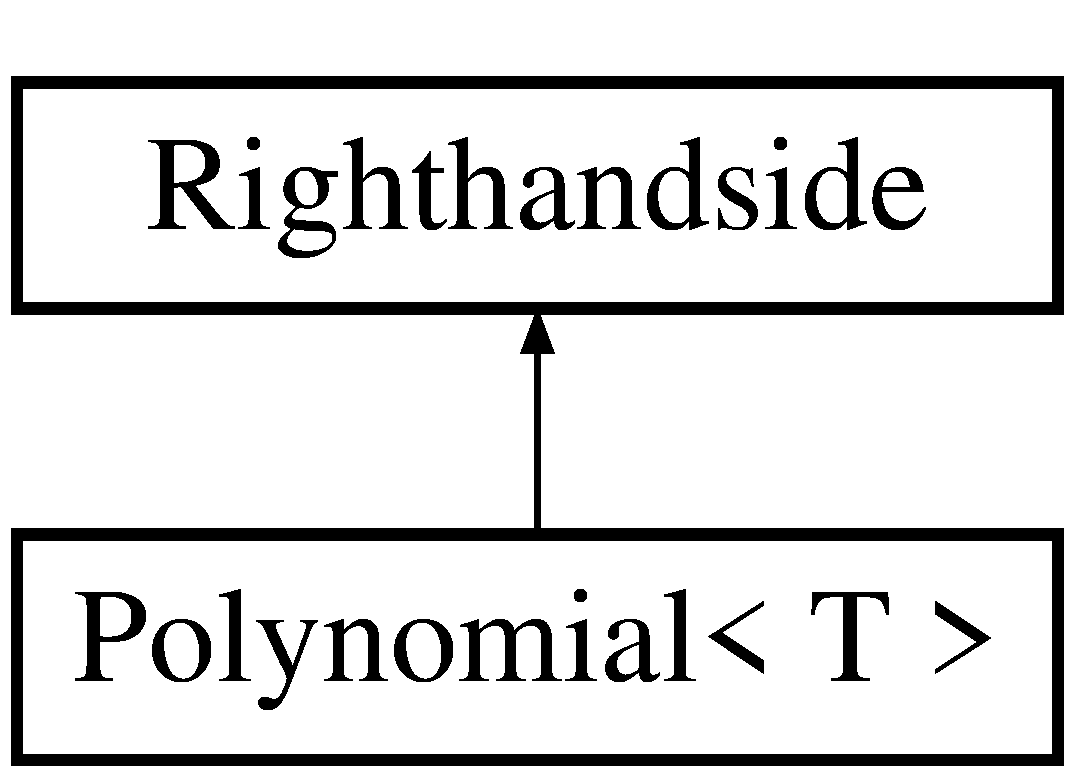
\includegraphics[height=2.000000cm]{class_polynomial}
\end{center}
\end{figure}
\subsection*{Public Member Functions}
\begin{DoxyCompactItemize}
\item 
\hypertarget{class_polynomial_a6b42d7b39422dac0a92b26a090bda215}{}\hyperlink{class_polynomial_a6b42d7b39422dac0a92b26a090bda215}{Polynomial} (T a1, T b1, T c1)\label{class_polynomial_a6b42d7b39422dac0a92b26a090bda215}

\begin{DoxyCompactList}\small\item\em Constructor for a polynomial of grade 2\+: a+b$\ast$x+c$\ast$x$^\wedge$2. \end{DoxyCompactList}\item 
\hypertarget{class_polynomial_a6d62fec5c43fe16ae174c43ae4c7b9ed}{}\hyperlink{class_polynomial_a6d62fec5c43fe16ae174c43ae4c7b9ed}{Polynomial} (T a1, T b1, T c1, T d1)\label{class_polynomial_a6d62fec5c43fe16ae174c43ae4c7b9ed}

\begin{DoxyCompactList}\small\item\em Constructor for a polynomial of grade 3\+: a+b$\ast$x+c$\ast$x$^\wedge$2+d$\ast$x$^\wedge$3. \end{DoxyCompactList}\item 
\hypertarget{class_polynomial_a3f959f3ca97a53a2d8a07e2db5153cc9}{}\hyperlink{class_polynomial_a3f959f3ca97a53a2d8a07e2db5153cc9}{Polynomial} (T a1, T b1, T c1, T d1, T e1)\label{class_polynomial_a3f959f3ca97a53a2d8a07e2db5153cc9}

\begin{DoxyCompactList}\small\item\em Constructor for a polynomial of grade 4\+: a+b$\ast$x+c$\ast$x$^\wedge$2+d$\ast$x$^\wedge$3+e$\ast$x$^\wedge$4. \end{DoxyCompactList}\item 
\hypertarget{class_polynomial_a31e8324c085875a18a39cdf67468fe69}{}virtual double \hyperlink{class_polynomial_a31e8324c085875a18a39cdf67468fe69}{value} (double y, double t) const \label{class_polynomial_a31e8324c085875a18a39cdf67468fe69}

\begin{DoxyCompactList}\small\item\em Virtual function to get the value of the function on the right hand side, f(y,t) for a specific y and t. \end{DoxyCompactList}\item 
\hypertarget{class_polynomial_a55c6a16f0e4ba0be54c8368cbffba28f}{}virtual double \hyperlink{class_polynomial_a55c6a16f0e4ba0be54c8368cbffba28f}{gradient} (double y, double t) const \label{class_polynomial_a55c6a16f0e4ba0be54c8368cbffba28f}

\begin{DoxyCompactList}\small\item\em Virtual function to get the value gradient of the function on the right hand side, f\textquotesingle{}(y,t) for a specific y and t. \end{DoxyCompactList}\end{DoxyCompactItemize}


\subsection{Detailed Description}
\subsubsection*{template$<$class T$>$class Polynomial$<$ T $>$}

\hyperlink{_polynomial_8hpp_source}{Polynomial.\+hpp}

Created on\+: Dic, 2015 \begin{DoxyVerb}Author: Francesco Mancino
\end{DoxyVerb}


Description\+: Derived class from \hyperlink{class_righthandside}{Righthandside}. Allow the user to specify a polynomial of grade 2 up to 4, in the form\+: a+b$\ast$x+c$\ast$x$^\wedge$2+d$\ast$x$^\wedge$3+e$\ast$x$^\wedge$4. The choice is given as to have int or double values for the coefficients with the the use of a template. 

The documentation for this class was generated from the following file\+:\begin{DoxyCompactItemize}
\item 
/\+Users/macair/\+Documents/projectode/Polynomial.\+hpp\end{DoxyCompactItemize}

\hypertarget{class_righthandside}{}\section{Righthandside Class Reference}
\label{class_righthandside}\index{Righthandside@{Righthandside}}


Abstract Base class of the family of possible right hand side functions f(y,t) in the O\+D\+E dy/dt=f(y,t).  




{\ttfamily \#include $<$Righthandside.\+hpp$>$}

Inheritance diagram for Righthandside\+:\begin{figure}[H]
\begin{center}
\leavevmode
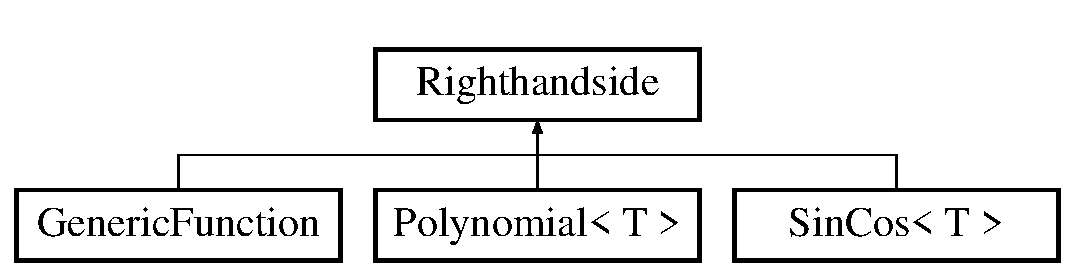
\includegraphics[height=2.000000cm]{class_righthandside}
\end{center}
\end{figure}
\subsection*{Public Member Functions}
\begin{DoxyCompactItemize}
\item 
\hypertarget{class_righthandside_ab9a7d9fb588db3cf6f0793dd3c610b21}{}void \hyperlink{class_righthandside_ab9a7d9fb588db3cf6f0793dd3c610b21}{Set\+Gradient\+Info} (bool a)\label{class_righthandside_ab9a7d9fb588db3cf6f0793dd3c610b21}

\begin{DoxyCompactList}\small\item\em Function to set the information about the gradient\+: if we have a gradient or not (going to be used inside the other classes). \end{DoxyCompactList}\item 
\hypertarget{class_righthandside_a789dc740ce5310a1ee78ca5ff19d965e}{}bool \hyperlink{class_righthandside_a789dc740ce5310a1ee78ca5ff19d965e}{Get\+Gradient\+Info} () const \label{class_righthandside_a789dc740ce5310a1ee78ca5ff19d965e}

\begin{DoxyCompactList}\small\item\em Function to get the information about the gradient. \end{DoxyCompactList}\item 
\hypertarget{class_righthandside_a6d32d90b10cecbcd7950f7cd1d9eea31}{}virtual double \hyperlink{class_righthandside_a6d32d90b10cecbcd7950f7cd1d9eea31}{value} (double y, double t) const  =0\label{class_righthandside_a6d32d90b10cecbcd7950f7cd1d9eea31}

\begin{DoxyCompactList}\small\item\em Virtual function to get the value of the function on the right hand side, f(y,t) for a specific y and t. \end{DoxyCompactList}\item 
\hypertarget{class_righthandside_a39748896cba8f34c145b46235ff2ee1a}{}virtual double \hyperlink{class_righthandside_a39748896cba8f34c145b46235ff2ee1a}{gradient} (double y, double t) const  =0\label{class_righthandside_a39748896cba8f34c145b46235ff2ee1a}

\begin{DoxyCompactList}\small\item\em Virtual function to get the value gradient of the function on the right hand side, f\textquotesingle{}(y,t) for a specific y and t. \end{DoxyCompactList}\end{DoxyCompactItemize}


\subsection{Detailed Description}
Abstract Base class of the family of possible right hand side functions f(y,t) in the O\+D\+E dy/dt=f(y,t). 

\hyperlink{_righthandside_8hpp_source}{Righthandside.\+hpp}

Created on\+: Dic, 2015 \begin{DoxyVerb}Author: Francesco Mancino
\end{DoxyVerb}


Description\+: Abstract class which is the head of the family of possible right hand side functions f(y,t) in the O\+D\+E dy/dt=f(y,t). The possible functions will be define as derived classes from this class. 

The documentation for this class was generated from the following files\+:\begin{DoxyCompactItemize}
\item 
/\+Users/macair/\+Documents/projectode/Righthandside.\+hpp\item 
/\+Users/macair/\+Documents/projectode/Righthandside.\+cpp\end{DoxyCompactItemize}

\hypertarget{class_runge_kutta4_solver}{}\section{Runge\+Kutta4\+Solver Class Reference}
\label{class_runge_kutta4_solver}\index{Runge\+Kutta4\+Solver@{Runge\+Kutta4\+Solver}}


Class that implements 4th order Runge-\/\+Kutta method to solve a O\+D\+E of the form\+: dy/dt=f(y,t).  




{\ttfamily \#include $<$Runge\+Kutta4\+Solver.\+hpp$>$}

Inheritance diagram for Runge\+Kutta4\+Solver\+:\begin{figure}[H]
\begin{center}
\leavevmode
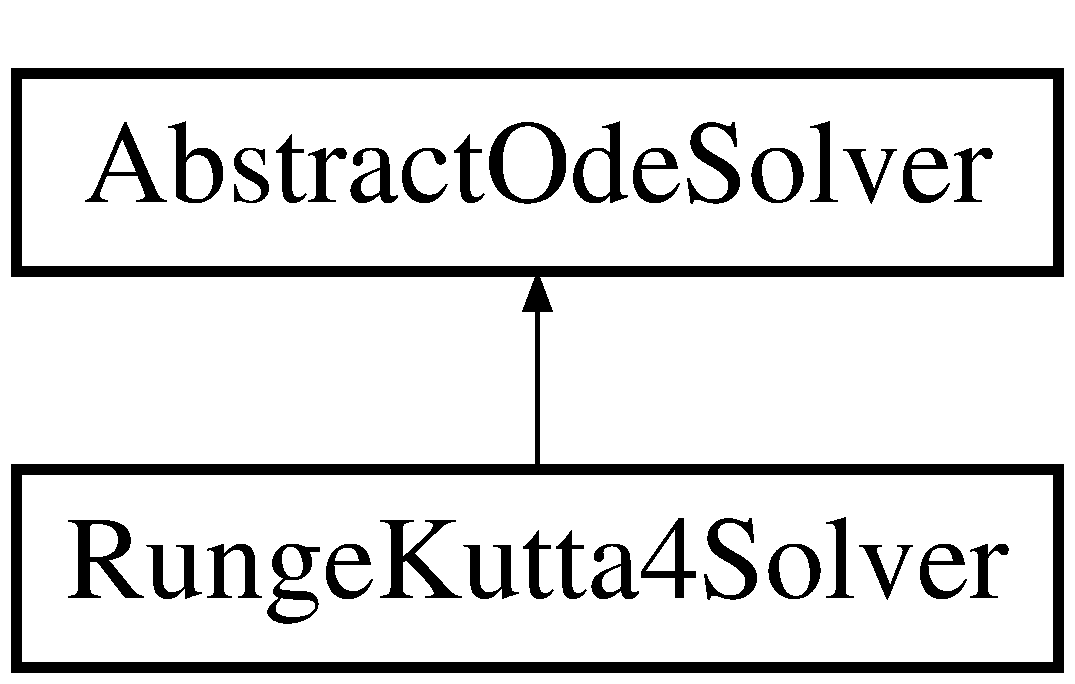
\includegraphics[height=2.000000cm]{class_runge_kutta4_solver}
\end{center}
\end{figure}
\subsection*{Public Member Functions}
\begin{DoxyCompactItemize}
\item 
virtual void \hyperlink{class_runge_kutta4_solver_acd37986ea1784f8ee4ae27f1614b06b8}{Solve\+Equation} (\hyperlink{class_righthandside}{Righthandside} $\ast$f, std\+::ostream \&stream)
\end{DoxyCompactItemize}


\subsection{Detailed Description}
Class that implements 4th order Runge-\/\+Kutta method to solve a O\+D\+E of the form\+: dy/dt=f(y,t). 

Runge\+Kutta4\+Solver.\+cpp

Created on\+: Dic, 2015 \begin{DoxyVerb}Author: Francesco Mancino
\end{DoxyVerb}


Description\+: Class that implements 4th order Runge-\/\+Kutta method to solve a O\+D\+E of the form\+: dy/dt=f(y,t). It is derived from the abstract class \hyperlink{class_abstract_ode_solver}{Abstract\+Ode\+Solver}. 

\subsection{Member Function Documentation}
\hypertarget{class_runge_kutta4_solver_acd37986ea1784f8ee4ae27f1614b06b8}{}\index{Runge\+Kutta4\+Solver@{Runge\+Kutta4\+Solver}!Solve\+Equation@{Solve\+Equation}}
\index{Solve\+Equation@{Solve\+Equation}!Runge\+Kutta4\+Solver@{Runge\+Kutta4\+Solver}}
\subsubsection[{Solve\+Equation(\+Righthandside $\ast$f, std\+::ostream \&stream)}]{\setlength{\rightskip}{0pt plus 5cm}void Runge\+Kutta4\+Solver\+::\+Solve\+Equation (
\begin{DoxyParamCaption}
\item[{{\bf Righthandside} $\ast$}]{f, }
\item[{std\+::ostream \&}]{stream}
\end{DoxyParamCaption}
)\hspace{0.3cm}{\ttfamily [virtual]}}\label{class_runge_kutta4_solver_acd37986ea1784f8ee4ae27f1614b06b8}
Virtual function the solves the O\+D\+E with initial conditions, Time interval, and number of steps specified in the methods of \char`\"{}\+Abstact\+Ode\+Solver\char`\"{}. The first input is the right hand side of the O\+D\+E, also a class, and the second input is the file in which the solution will be saved. 

Implements \hyperlink{class_abstract_ode_solver_ad7d73b20e9ce5c8f3aab1a15bebe3e4c}{Abstract\+Ode\+Solver}.



The documentation for this class was generated from the following files\+:\begin{DoxyCompactItemize}
\item 
/\+Users/macair/\+Documents/projectode/Runge\+Kutta4\+Solver.\+hpp\item 
/\+Users/macair/\+Documents/projectode/Rungekutta4\+Solver.\+cpp\end{DoxyCompactItemize}

\hypertarget{class_sin_cos}{}\section{Sin\+Cos$<$ T $>$ Class Template Reference}
\label{class_sin_cos}\index{Sin\+Cos$<$ T $>$@{Sin\+Cos$<$ T $>$}}


Class that allows the user to specify a function of the type f(y,t)=a$\ast$sin(c$\ast$y)+b$\ast$cos(d$\ast$y) for the right hand side of the O\+D\+E.  




{\ttfamily \#include $<$Sin\+Cos.\+hpp$>$}

Inheritance diagram for Sin\+Cos$<$ T $>$\+:\begin{figure}[H]
\begin{center}
\leavevmode
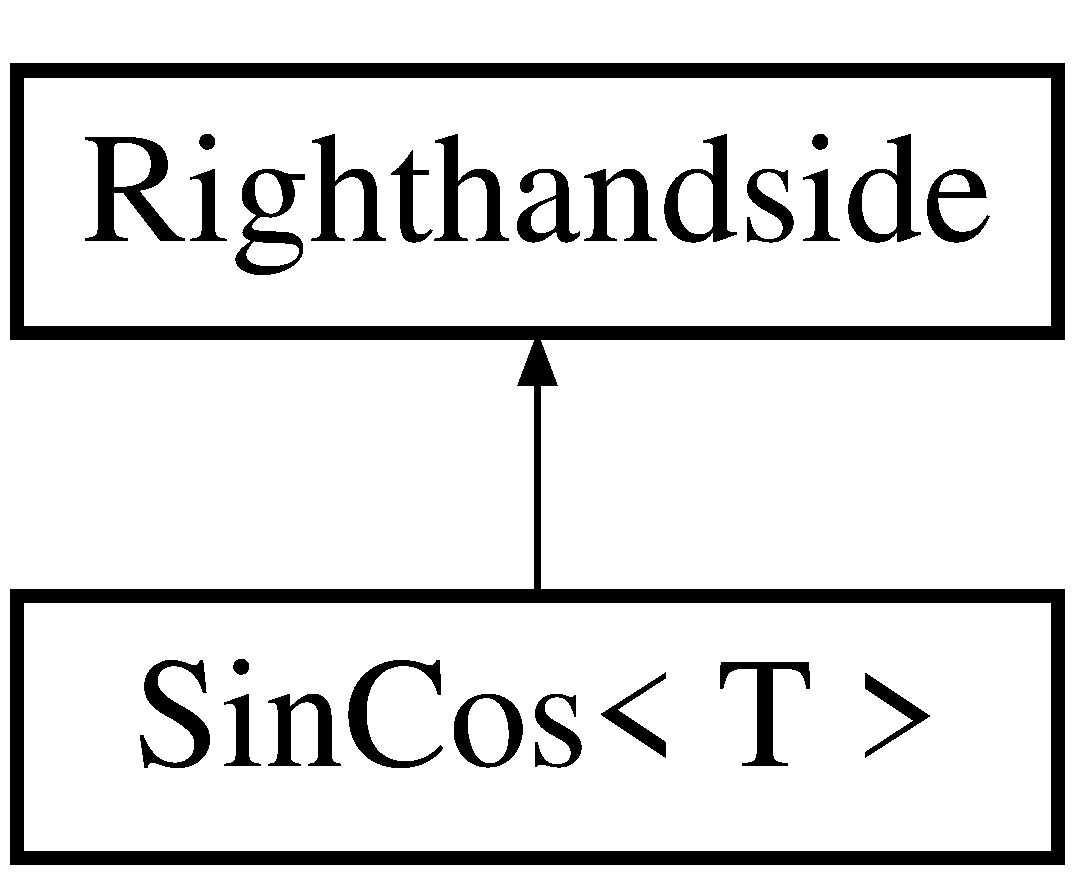
\includegraphics[height=2.000000cm]{class_sin_cos}
\end{center}
\end{figure}
\subsection*{Public Member Functions}
\begin{DoxyCompactItemize}
\item 
\hypertarget{class_sin_cos_a3cac71427371707bdab285bdd397aa3d}{}\hyperlink{class_sin_cos_a3cac71427371707bdab285bdd397aa3d}{Sin\+Cos} (T a1)\label{class_sin_cos_a3cac71427371707bdab285bdd397aa3d}

\begin{DoxyCompactList}\small\item\em Constructor for a sine function \+: a$\ast$sin(y) (for constructing a pure cosine function it is possible to call \hyperlink{class_sin_cos}{Sin\+Cos(0,1)}) \end{DoxyCompactList}\item 
\hypertarget{class_sin_cos_a64e4afd2a47fa1375b101b2e439be409}{}\hyperlink{class_sin_cos_a64e4afd2a47fa1375b101b2e439be409}{Sin\+Cos} (T a1, T b1)\label{class_sin_cos_a64e4afd2a47fa1375b101b2e439be409}

\begin{DoxyCompactList}\small\item\em Constructor for a function of the type\+: a$\ast$sin(y)+b$\ast$cos(y) \end{DoxyCompactList}\item 
\hypertarget{class_sin_cos_a922f7496fd03a8429fd96e29ba21fa64}{}\hyperlink{class_sin_cos_a922f7496fd03a8429fd96e29ba21fa64}{Sin\+Cos} (T a1, T b1, T c1, T d1)\label{class_sin_cos_a922f7496fd03a8429fd96e29ba21fa64}

\begin{DoxyCompactList}\small\item\em Constructor for a function of the type\+: f(y,t)=a$\ast$sin(c$\ast$y)+b$\ast$cos(d$\ast$y) \end{DoxyCompactList}\item 
\hypertarget{class_sin_cos_a2ccce937dae380440f1278f8c0f5801c}{}virtual double \hyperlink{class_sin_cos_a2ccce937dae380440f1278f8c0f5801c}{value} (double y, double t) const \label{class_sin_cos_a2ccce937dae380440f1278f8c0f5801c}

\begin{DoxyCompactList}\small\item\em Virtual function to get the value of the function on the right hand side, f(y,t) for a specific y and t. \end{DoxyCompactList}\item 
\hypertarget{class_sin_cos_abed60e185e8838cf409613152af45ee9}{}virtual double \hyperlink{class_sin_cos_abed60e185e8838cf409613152af45ee9}{gradient} (double y, double t) const \label{class_sin_cos_abed60e185e8838cf409613152af45ee9}

\begin{DoxyCompactList}\small\item\em Virtual function to get the value gradient of the function on the right hand side, f\textquotesingle{}(y,t) for a specific y and t. \end{DoxyCompactList}\end{DoxyCompactItemize}


\subsection{Detailed Description}
\subsubsection*{template$<$class T$>$class Sin\+Cos$<$ T $>$}

Class that allows the user to specify a function of the type f(y,t)=a$\ast$sin(c$\ast$y)+b$\ast$cos(d$\ast$y) for the right hand side of the O\+D\+E. 

\hyperlink{_sin_cos_8hpp_source}{Sin\+Cos.\+hpp}

Created on\+: Dic, 2015 \begin{DoxyVerb}Author: Francesco Mancino
\end{DoxyVerb}


Description\+: Derived class from \hyperlink{class_righthandside}{Righthandside}. Contructs a function of the type\+: f(y,t)=a$\ast$sin(c$\ast$y)+b$\ast$cos(d$\ast$y) 

The documentation for this class was generated from the following file\+:\begin{DoxyCompactItemize}
\item 
/\+Users/macair/\+Documents/projectode/Sin\+Cos.\+hpp\end{DoxyCompactItemize}

\hypertarget{class_three_step_solver}{}\section{Three\+Step\+Solver Class Reference}
\label{class_three_step_solver}\index{Three\+Step\+Solver@{Three\+Step\+Solver}}


{\ttfamily \#include $<$Three\+Step\+Solver.\+hpp$>$}

Inheritance diagram for Three\+Step\+Solver\+:\begin{figure}[H]
\begin{center}
\leavevmode
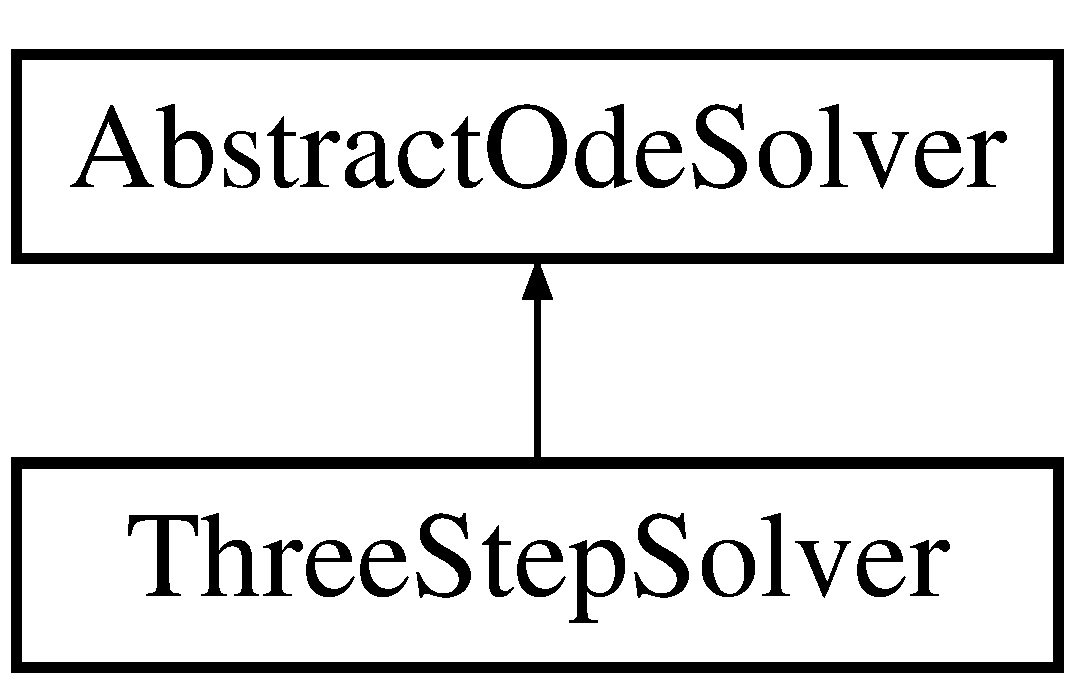
\includegraphics[height=2.000000cm]{class_three_step_solver}
\end{center}
\end{figure}
\subsection*{Public Member Functions}
\begin{DoxyCompactItemize}
\item 
virtual void \hyperlink{class_three_step_solver_a5c84debbe6e3497ab3c4b796e1f92cee}{Solve\+Equation} (\hyperlink{class_righthandside}{Righthandside} $\ast$f, std\+::ostream \&stream)
\end{DoxyCompactItemize}


\subsection{Detailed Description}
Trhee\+Step\+Solver.\+cpp

Created on\+: Dic, 2015 \begin{DoxyVerb}Author: Francesco Mancino
\end{DoxyVerb}


Description\+: Class that implements Three Step Adam Bashworts Method to solve a O\+D\+E of the form\+: dy/dt=f(y,t). It is derived from the abstract class \hyperlink{class_abstract_ode_solver}{Abstract\+Ode\+Solver}. 

\subsection{Member Function Documentation}
\hypertarget{class_three_step_solver_a5c84debbe6e3497ab3c4b796e1f92cee}{}\index{Three\+Step\+Solver@{Three\+Step\+Solver}!Solve\+Equation@{Solve\+Equation}}
\index{Solve\+Equation@{Solve\+Equation}!Three\+Step\+Solver@{Three\+Step\+Solver}}
\subsubsection[{Solve\+Equation(\+Righthandside $\ast$f, std\+::ostream \&stream)}]{\setlength{\rightskip}{0pt plus 5cm}void Three\+Step\+Solver\+::\+Solve\+Equation (
\begin{DoxyParamCaption}
\item[{{\bf Righthandside} $\ast$}]{f, }
\item[{std\+::ostream \&}]{stream}
\end{DoxyParamCaption}
)\hspace{0.3cm}{\ttfamily [virtual]}}\label{class_three_step_solver_a5c84debbe6e3497ab3c4b796e1f92cee}
Virtual function the solves the O\+D\+E with initial conditions, Time interval, and number of steps specified in the methods of \char`\"{}\+Abstact\+Ode\+Solver\char`\"{}. The first input is the right hand side of the O\+D\+E, also a class, and the second input is the file in which the solution will be saved. 

Implements \hyperlink{class_abstract_ode_solver_ad7d73b20e9ce5c8f3aab1a15bebe3e4c}{Abstract\+Ode\+Solver}.



The documentation for this class was generated from the following files\+:\begin{DoxyCompactItemize}
\item 
/\+Users/macair/\+Documents/projectode/Three\+Step\+Solver.\+hpp\item 
/\+Users/macair/\+Documents/projectode/Three\+Step\+Solver.\+cpp\end{DoxyCompactItemize}

\hypertarget{class_two_step_solver}{}\section{Two\+Step\+Solver Class Reference}
\label{class_two_step_solver}\index{Two\+Step\+Solver@{Two\+Step\+Solver}}


{\ttfamily \#include $<$Two\+Step\+Solver.\+hpp$>$}

Inheritance diagram for Two\+Step\+Solver\+:\begin{figure}[H]
\begin{center}
\leavevmode
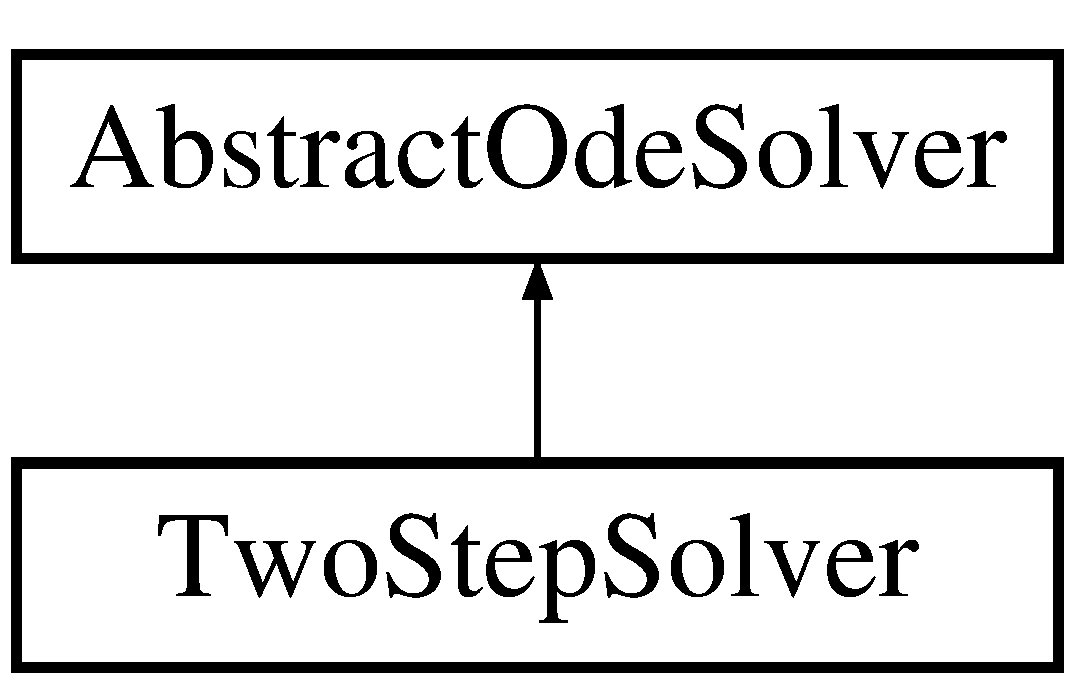
\includegraphics[height=2.000000cm]{class_two_step_solver}
\end{center}
\end{figure}
\subsection*{Public Member Functions}
\begin{DoxyCompactItemize}
\item 
virtual void \hyperlink{class_two_step_solver_ae52e8c2313e8f9fa617d13b7ed83284e}{Solve\+Equation} (\hyperlink{class_righthandside}{Righthandside} $\ast$f, std\+::ostream \&stream)
\end{DoxyCompactItemize}


\subsection{Detailed Description}
\hyperlink{_two_step_solver_8hpp_source}{Two\+Step\+Solver.\+hpp}

Created on\+: Dic, 2015 \begin{DoxyVerb}Author: Francesco Mancino
\end{DoxyVerb}


Description\+: Class that implements Two Step Adam Bashworts Method to solve a O\+D\+E of the form\+: dy/dt=f(y,t). It is derived from the abstract class \hyperlink{class_abstract_ode_solver}{Abstract\+Ode\+Solver}. 

\subsection{Member Function Documentation}
\hypertarget{class_two_step_solver_ae52e8c2313e8f9fa617d13b7ed83284e}{}\index{Two\+Step\+Solver@{Two\+Step\+Solver}!Solve\+Equation@{Solve\+Equation}}
\index{Solve\+Equation@{Solve\+Equation}!Two\+Step\+Solver@{Two\+Step\+Solver}}
\subsubsection[{Solve\+Equation(\+Righthandside $\ast$f, std\+::ostream \&stream)}]{\setlength{\rightskip}{0pt plus 5cm}void Two\+Step\+Solver\+::\+Solve\+Equation (
\begin{DoxyParamCaption}
\item[{{\bf Righthandside} $\ast$}]{f, }
\item[{std\+::ostream \&}]{stream}
\end{DoxyParamCaption}
)\hspace{0.3cm}{\ttfamily [virtual]}}\label{class_two_step_solver_ae52e8c2313e8f9fa617d13b7ed83284e}
Virtual function the solves the O\+D\+E with initial conditions, Time interval, and number of steps specified in the methods of \char`\"{}\+Abstact\+Ode\+Solver\char`\"{}. The first input is the right hand side of the O\+D\+E, also a class, and the second input is the file in which the solution will be saved. 

Implements \hyperlink{class_abstract_ode_solver_ad7d73b20e9ce5c8f3aab1a15bebe3e4c}{Abstract\+Ode\+Solver}.



The documentation for this class was generated from the following files\+:\begin{DoxyCompactItemize}
\item 
/\+Users/macair/\+Documents/projectode/Two\+Step\+Solver.\+hpp\item 
/\+Users/macair/\+Documents/projectode/Two\+Step\+Solver.\+cpp\end{DoxyCompactItemize}

%--- End generated contents ---

% Index
\backmatter
\newpage
\phantomsection
\clearemptydoublepage
\addcontentsline{toc}{chapter}{Index}
\printindex

\end{document}
